\documentclass{article}
\usepackage{amsmath}
\usepackage{amssymb}
\usepackage{graphicx}
\usepackage{hyperref}
\usepackage[version=4]{mhchem}

\title{Problem 3}
\date{}

\begin{document}
\maketitle

\section*{Problem}
In scalene triangle \(A B C, A Q=P Q, M P=P N, P M \perp A B, P N \perp A C\). The correct one of the followings is\\
(1) \(A N=A M\);\\
(2) \(Q P / / A M\);\\
(3) \(\triangle B M P \cong \triangle Q N P\).\\
(A) all are correct\\
(B) only (1) and (2) are correct\\
(C) only (2) and (3) are correct\\
(D) only (1) is correct\\
(E) none is correct\\
\centering
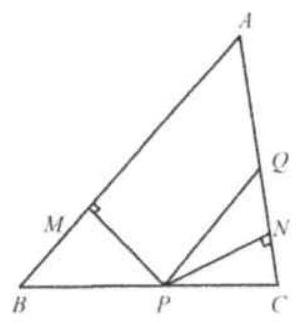
\includegraphics[width=\textwidth]{images/problem_image_1.jpg}

\section*{Solution}
(B).
Connect \(A P\). Since \(M P=P N\) and \(P M \perp A B, A P\) is the angle bisector of \(\angle A\). We also know that \(A Q=P Q\).\\
So \(\angle A P Q=\angle Q A P=\angle P A M=\alpha\).\\
Thus, \(Q P / / A M\).\\
Since \(\triangle A P M\) and \(\triangle A P N\) are congruent \((A N=A M, M P=P N\), and \(\angle A M P=\angle A N P=90^{\circ}\) ),\\
\centering
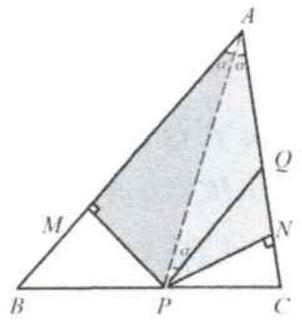
\includegraphics[width=\textwidth]{images/reasoning_image_1.jpg}


So \(A N=A M\).\\
If \(\triangle B M P \cong \triangle Q N P\), then \(B P-P Q=A Q, \angle B=\angle Q P C=\angle P Q C\). Then we will have \(P C=Q C, B C=A C\). Triangle \(A B C\) is not a scalene triangle anymore.\\
So only (1) and (2) are correct.

\end{document}
